\section{MHD}


\begin{frame}{BLH model + superimposed $\vec{B}$}

\begin{minipage}[t]{0.48\textwidth}
\vspace{0pt}
        \begin{figure}
                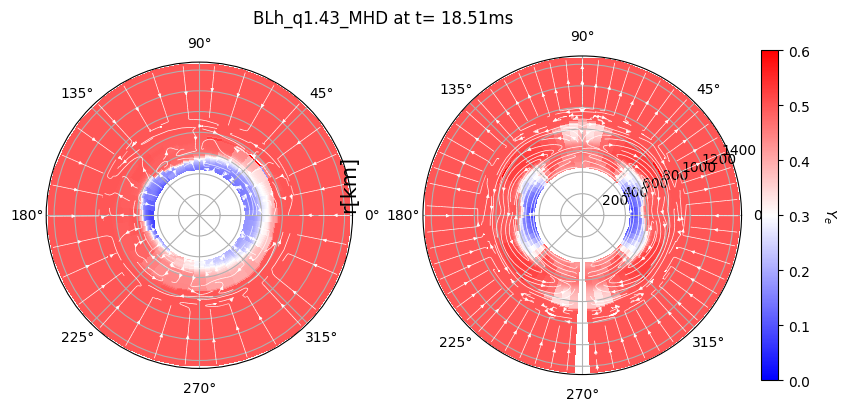
\includegraphics[width=1.1\linewidth]{../fig/blh_vlr_hr_constatm_mhd/ye_bfield.png}

        \end{figure}

\end{minipage}
\hfill
\begin{minipage}[t]{0.45\textwidth}
\vspace{0pt}
\begin{tcolorbox}[
    colback=white,
    colframe=blue,
    colbacktitle=blue!50!black!50,
    title=Ongoing,
    fonttitle=\bfseries,
    rounded corners,
    boxrule=1pt,
    left=2mm, right=2mm, top=1mm, bottom=1mm
]
\begin{itemize}
   \scriptsize 
    \item 1st simulation on-going
    \item Better termalization of charged particles such as $\alpha$
    \item Correlations of B field ?
    \item Is B stronger at equator(low-ye)/poles(high-ye)?
    \item Does it matter for nucleosynthesis and light curves?

	
\end{itemize}
\end{tcolorbox}
\end{minipage}

\end{frame}


